\documentclass[12pt,a4]{article}

\usepackage[utf8]{inputenc}
\usepackage[T1]{fontenc}
\usepackage{amsmath,amsfonts}
\usepackage{mathtools}
\usepackage{graphicx}
\usepackage{enumerate}
\DeclareMathOperator*{\argmin}{\arg\!\min}

\newcommand{\R}{{\mathbb R}}
\newcommand{\C}{{\mathbb C}}
\newcommand{\N}{{\mathbb N}}
\newcommand{\ra}{\rightarrow}
\newcommand{\lra}{\longrightarrow}
\newcommand{\lnorm}{\left\|}
\newcommand{\rnorm}{\right\|}
\newcommand{\ind}{{\mathbf{1}}}

\newcommand{\citeneeded}{\ensuremath{\vphantom{1}^{\text{[citation needed]}}\,}}
\newcommand{\eps}{\ensuremath{\varepsilon}}


\title{Glottal inversion with an approximate vocal tract filter}
\author{Lasse Lybeck, Robert Sirviö}


\begin{document}

\maketitle

%---------------------Introduction--------------------
\section{Introduction}\label{sec:intro}

A synthetic human vowel sound consists of a periodic signal to simulate the glottal excitation signal at the glottis and a filter to simulate the vocal tract, which the glottal signal is filtered through.\cite{touda} With a given vocal tract filter the direct problem is \emph{given a glottal excitation signal, create the vowel sound}. The inverse problem is \emph{given a (recorded) vowel sound, find the glottal excitation signal}. In this study we will be concentrating on the inverse problem using simulated vowel data.

The inversion from a vowel sound to the glottal signal is an important part of creating synthetic human voices and speech generators. To create a synthetic vowel both the glottal signal and the vocal tract filter are needed. However, the glottal signal cannot be directly measured, but it can be approximated with inversion of a recorded vowel. With this data models for simulating the glottal excitation signal can be created.


%-----------------Materials & Methods-----------------
\section{Materials and Methods}\label{sec:methods}

\subsection{Glottal excitation signal}
\label{sec:rk}

In this study the Rosenberg-Klatt model (RK-model) for the glottal excitation signal will be used for the generation of synthetic data and as a reference point for the obtained results. The RK-model is a simple model for the glottal signal, proposed in 1970 by Rosenberg.\cite{rosenberg} The model is simple and easy to use, as it creates the signal only from two parameters, the sound frequency $f$ and the so called Klatt-parameter $Q$.

The \emph{airflow} for the glottal excitation signal created by the RK-model is defined as
\begin{equation}
\label{eq:RK-model}
g(t) =
  \begin{cases}
   at^2 + bt^3  & \text{if } 0 \leq t \leq Q T \\
   0            & \text{if } Q T < t \leq T,
  \end{cases}
\end{equation}
where $t$ is a time variable, $T = 1/f$ is the period of the pitch, $Q \in \left[ 0,1 \right]$ is the Klatt-parameter and $a$ and $b$ are variables defined in terms of $T_0 := QT$ as
\begin{equation*}
a = \frac{27}{4 T_0^2}, \quad b = -\frac{27}{4 T_0^3} .
\end{equation*}
Here the parameter $f$ defines the frequency of the generated signal and the Klatt-parameter $Q$ defines the shape of the pulse.

The glottal excitation signal can be retrieved as the derivative $g'$ of the airflow function. Here $g'$ is the \emph{pressure function}, and simulates the sound generated in the glottis. The pulse generated by the model can be seen in figure \ref{fig:klatt}.

Another, more widely used, model for the glottal excitation signal worth mentioning is the Liljencrants-Fant model (LF-model).\cite{fant} It is regarded as more accurate than the RK-model, but it is also much more complex. It has also been shown, that the LF-model generates only marginally better approximations for the resulting vowel after the vocal tract filtering than the RK-model.\cite{fujisaki} Due to this and the overall complexity of the LF-model we will be using the RK-model for the simulation of the glottal excitation signal in this study.

\begin{figure}[t]
\begin{center}
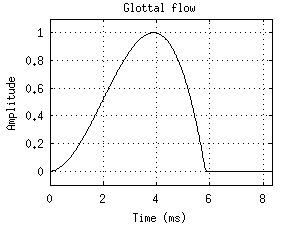
\includegraphics[scale=1]{img/klattflow.png}
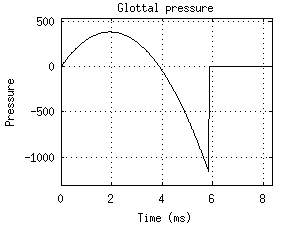
\includegraphics[scale=1]{img/klattpres.png}
\end{center}
\caption{The airflow and pressure generated by the RK-model}
\label{fig:klatt}
\end{figure}


\subsection{Vocal tract filter}
\label{sec:filter}

In this study we will assume an approximate vocal tract filter to be known for the recorded vowel we want to invert. The digital filter, defined by a vector $a \in \R^{N_a}$, filters the data $x \in \R^n$ as defined by the difference equation
\begin{equation}
\left\{
\begin{alignedat}{1}
\label{eq:filter-diffeq}
y_1     &= x_1 \\
a_1 y_j &= -\sum_{k=2}^{\min\{j-1, N_a\}} a_{k} y_{j-k} ,
\end{alignedat}
\right.
\end{equation}
where $y \in \R^n$ is the filtered data. We denote $y = \varphi_a (x)$.

Consider now the filter defined by $a \in \R^{N_a}$ and the data $x \in \R_n$ which we want to filter. Now the filter defined by \eqref{eq:filter-diffeq} can be expressed by the the matrix $A \in \R^{n \times n}$, where
\begin{equation}
\label{eq:filter-matrix}
\left\{
\begin{alignedat}{3}
   &A_{1,1}     = a_1 \\
   &A_{i,1}     = - \sum_{k=1}^{\min\{ i-1, N_a-1 \}} a_{k+1} A_{i-k,1}, \quad && 2 \leq i \leq n \\
   &A_{i+1,j+1} = A_{i,j},     && j \leq i \\
   &A_{i,j}     = 0,           && j > i .
\end{alignedat}
\right.
\end{equation}
Now $\varphi_a (x) = Ax$.


\subsection{The matrix model}
\label{sec:matrixModel}

A vowel sound can be simulated by applying a digital filter $A \in \R^{n \times n}$, defined as in \eqref{eq:filter-matrix}, to a sample of a glottal excitation signal $g \in \R^n$ as
\begin{equation}
\label{eq:vow}
v = A g .
\end{equation}
Here $v \in \R^n$ is the simulated vowel.

In this study we will assume an approximation of the filter $A$ to be known. Given the measurement $m \in \R^n$ of a vowel corresponding approximately to the filter $A$, equation \eqref{eq:vow} can be expressed as
\begin{equation}
\label{eq:vowModel}
m = A g + \eps,
\end{equation}
where $\eps \in \R^n$ denotes the measurement noise.


\subsection{The inversion method}\label{sec:invMethod}

\subsubsection{Tikhonov reguralization}\label{sec:tikh}
The classical Tikhonov regularized solution for $m = Ag + \varepsilon$, defined in section \ref{sec:matrixModel}, is usually denoted by the vector $T_\alpha(m)\in\R^n$ that minimizes
\begin{equation*}
\lnorm AT_\alpha(m) - m \rnorm^2 + \alpha \lnorm T_\alpha(m) \rnorm^2 \Leftrightarrow
\end{equation*}
\begin{equation*}
T_\alpha(m) = \underset{z\in\R^n}{\argmin}
\left\{ \lnorm Az - m \rnorm^2 + \alpha \lnorm z \rnorm^2 \right\},
\end{equation*}
where $\alpha > 0$ is called a regularization parameter. The resulting $T_\alpha(m)$ can be understood as a compromise between two conditions, namely
\begin{enumerate}[I.]
 \item $T_\alpha(m)$ should give a small residual $AT_\alpha(m) - m$.
 \item $\lnorm T_\alpha(m) \rnorm_2$ should be small.
\end{enumerate}
The $\alpha$ parameter is used in order to tune to balance between the two conditions above.

In generalized Tikhonov regularization some prior knowledge is assumed to be known. For example, in some cases $g$ might be known to be smooth. This information can be incorporated into the regularization by choosing
\begin{equation}
T_\alpha(m) = \underset{z\in\R^n}{\argmin}
\left\{ \lnorm Az - m \rnorm^2 + \alpha \lnorm Lz \rnorm^2 \right\},
\end{equation}  
where $L$ is a discretized differential operator. As shown in \cite{samu}, the regularized solution satisfies
\begin{equation}
\label{eq:tik-normal}
\left( A^T A + \alpha L^T L \right) T_{\alpha}(m) = A^T m ,
\end{equation}
which can be used to calculate the solution numerically.
 
In our model proposed in section \ref{sec:rk} we know the airflow of the excitation signal to be smooth in the interval $[0, QT]$ and to be zero in the interval $]QT, T]$. This can be incorporated in our model by customizing the discrete differential operator matrix, described in more detail in section \ref{sec:basis}.


\subsubsection{The conjugate gradient method}
\label{sec:conjgrad}

The conjugate gradient method is an iterative method for the quadratic optimization problem
\begin{equation}
\label{eq:quad-optim}
\text{minimize } \frac{1}{2} x^T Q x - b^T x ,
\end{equation}
where $Q \in \R^{n \times n}$ is a symmetric positive definite matrix. We will now briefly explain the algorithm and its use to our particular problem. For a more detailed explanation, see \cite{samu}.

Let $b \in \R^n$ fixed, $Q \in \R^{n \times n}$ a symmetric positive definite matrix, $x_0 \in \R^n$ the initial guess and define $d_0 = -g_0 = b - Q x_0$. Now for $k \geq 0$ let
\begin{equation}
\begin{alignedat}{1}
\alpha_k &= \frac{g_k^T d_k}{d_k^T Q d_k} \\
x_{k+1}  &= x_k + \alpha_k d_k \\
g_{k+1}  &= Q x_{k+1} - b \\
\beta_k  &= \frac{g_{k+1}^T Q d_k}{d_k^T Q d_k} \\
d_{k+1}  &= -g_{k+1} + \beta_k d_k .
\end{alignedat}
\end{equation}
Now $x_k$ converges toward the solution of \eqref{eq:quad-optim}. We now want to apply the conjugate gradient algorithm in the case of the optimization problem defined in \eqref{eq:tik-normal} for the Tikhonov regularization.

Let $A \in \R^{n \times n}$, $L \in R^{n \times n}$ invertible and $\alpha > 0$. Now the square matrix $B := A^T A + \alpha L^T L$ is invertible. If we denote $f := T_\alpha (m)$ in \eqref{eq:tik-normal}, the problem becomes to minimize the expression
\begin{equation}
\label{eq:conjgrad-basis}
\lnorm B f - A^T m \rnorm^2 .
\end{equation}

We see that
\begin{equation}
\label{eq:conjgrad-calc}
\begin{alignedat}{1}
\lnorm B f - A^T m \rnorm^2
  &= \left< Bf, Bf \right> - 2 \left< Bf, A^T m \right> + \left< A^T m, A^T m \right> \\
  &= f^T B^T B f - 2 m^T A B f + \lnorm A^T m \rnorm^2 .
\end{alignedat}
\end{equation}
Further, we notice that $B^T B$ is a positive definite symmetric matrix, since
\begin{equation*}
v^T (B^T B) v = (B v)^T B v = \lnorm B v \rnorm^2 > 0
\end{equation*}
for any $v \in R^n$, $v \neq 0$, due to the fact that $B$ is invertible. Now we define
\begin{equation*}
Q := 2 B^T B \quad \text{and} \quad b^T := 2 m^T A B .
\end{equation*}
As can be seen from \eqref{eq:conjgrad-calc}, minimizing \eqref{eq:conjgrad-basis} is equivalent to minimizing the expression
\begin{equation}
\frac{1}{2} f^T Q f - b^T f ,
\end{equation}
and thus we can use the conjugate gradient method for the optimization.



\subsubsection{Morozov's discrepancy principle}
The problem of finding the optimal regularization parameter is, in general, considered to be unsolved. There are, however, methods that attempt to find an optimal choice of the regularization parameter, including the Mozorov discrepancy principle, which is based on the noise level in the data.

Assume that we know the size of the noise in our model defined by \eqref{eq:vowModel} to be $\delta > 0$. Now $T_\alpha(m)$ is an acceptable reconstruction if 
\begin{equation}
\lnorm AT_\alpha(m)-m\rnorm \leq \delta \quad \left( A \in R^{k \times n}\right).
\end{equation}
If we assume that 
\begin{equation}
\eps = \left(\eps_1, \ldots, \eps_n\right)\in\R^n, \quad \eps_k \sim N\left(0,1\right) \text{ for all } k\in\left\{1, \ldots, n\right\},
\end{equation}
we can choose $\delta = \sqrt{n}$ since $E\left(\lnorm \eps \rnorm\right) = \sqrt{n}.$

The idea of the Morozov's discrepancy principle is to choose $\alpha > 0$ such that
\begin{equation}
\lnorm AT_\alpha(m) - m \rnorm = \delta
\end{equation}
It can be proven (see \cite{samu}) that the $\alpha$ that satisfies the above expression is attained by solving
\begin{equation}
\sum_{j=1}^{\min\left\{ k,n \right\}} \left( \frac{\alpha}{d_j^2 + \alpha} \right)^2 \left( m'_j \right)^2 + \sum_{j = \min\left\{k,n\right\} + 1}^k \left( m'_j \right)^2 - \delta^2 = 0,
\end{equation}
where $d_j$ are the singular values of $A$ and $m' = U^Tm$ where $U$ is an orthogonal matrix acquired from the singular value decomposition $A=UDV^T$.


\subsection{The basis and materials}\label{sec:basis}

In this work we will use synthetic data as our basis. We first create a synthetic glottal excitation signal using the airflow function defined in \eqref{eq:RK-model}. To this signal we apply a previously calculated vocal tract filter, as described in section \ref{sec:filter} to create a simulated vowel sound. Finally we add some normally distributed noise to the data to simulate measurement noise. Different data is created by varying the sound frequency, the value of the Klatt-parameter $Q$ and the noise-level.

The inversion of the vowel sound is done using another filter similar to the one used in creating the synthetic data. For example we might have created the data with a filter for a male vowel /a/, and use a filter for a female vowel /a/ for the inversion. This way we avoid inverse crime. The idea is that we can assume two different filters for the same vowel to be approximately the same. That is, given two different filters $A_1$ and $A_2$ for the same vowel and a glottal excitation signal $g$, we assume that $A_1 g \approx A_2 g$. This is based on the fact that a vowel is defined by its two or three first \emph{formant frequencies}, which can be assumed to be about the same for two different vowel sounds.\cite{digitalmodels}

We then attempt to solve the inverse problem by using the generalized Tikhonov regularization with a customized penalty matrix. We will assume the Klatt-parameter $Q$ of the glottal excitation signal to be known (at least approximately), and as explained in section \ref{sec:rk} we know the pressure function to be zero in the interval $]QT, T]$. This will be incorporated in the model by assigning large values to the diagonal entries $l_i \in L$ for the values of $i$ that correspond to the previously mentioned interval, namely $i \in \left\{ j \in \N : Qn < j \leq n \right\}$ where $n$ is the length of our data. We also know the pressure function to be smooth in the interval $[0, Q]$. This can be incorporated by adding differential operator properties to the penalty matrix.

We can thus assign the differential operator properties
\begin{equation*}
\begin{cases}
 l_{i,i}   &= 1 \\
 l_{i,i+1} &= -1 
\end{cases}
\text{ when } i \in \left\{ j \in \N : 1 \leq j \leq Qn \right\} ,
\end{equation*}
and further, we can for example assign the larger values described above as
\begin{equation*}
 l_{i,i} = 10, \quad \text{when } i \in \left\{ j \in \N : Qn < j \leq n \right\}
\end{equation*}
resulting in the penalty matrix
\begin{equation}
L=
\begin{pmatrix*}[c]
 1      & -1     &  0     & 0       &    &    & \cdots  &        & 0       \\
 0      & 1      & -1     & 0       &    &    & \cdots  &        & 0       \\
 \vdots &        & \ddots & \ddots  &    &    &         &        & \vdots  \\
 0      & \cdots &  0     & 1       & -1 & 0  & 0       & \cdots & 0       \\
 0      & \cdots &  0     & 0       & 10 & 0  & 0       & \cdots & 0       \\
 0      & \cdots &  0     & 0       & 0  & 10 & 0       & \cdots & 0       \\
 \vdots &        &        &         &    &    & \ddots  &        & \vdots  \\
 0      &        &        & \cdots  &    &    &  0      &  10    & 0       \\
 0      &        &        & \cdots  &    &    &  0      &  0     & 10 
\end{pmatrix*}
\end{equation}
for a single period of the excitation signal. This procedure must of course be repeated as many times as we have periods in our measurement data.



%-----------------------Results-----------------------
\section{Results}\label{sec:results}


%----------------------Discussion---------------------
\section{Discussion}\label{sec:discussion}

\newpage
\begin{thebibliography}{9}

\bibitem{fant}
    Fant, G., Liljencrants, J., Lin, Q., (1985).
    \emph{A four-parameter model of glottal flow}.
    STL-QPSR 26 (4), p. 1-13
    
\bibitem{fujisaki}
    Fujisaki, H., Ljungqvist, M., 1986.
    Proposal and evaluation of models for the glottal source waveform.
    In: Proc. IEEE International Conference on Acoustics, Speech and Signal Processing (ICASSP). Vol. 11. p. 1605–1608.
    
\bibitem{samu}
	Mueller, Jennifer L. \& Siltanen Samuli, (2012).
	\emph{Linear and Nonlinear Inverse Problems with Practical Applications}.
	SIAM, 1:st edition.
	
\bibitem{touda}
    Touda, K., (2007)
    \emph{Study on numerical method for voice generation problem}.
    PhD thesis.
    The University of Electro-Communications.
    
\bibitem{digitalmodels}
    Rabiner, L. R., Schafer, R. W., (1987).
    \emph{Digital processing of speech signals}.
    Englewood Cliffs: Prentice-Hall, p. 38-107.

\bibitem{rosenberg}
    Rosenberg, A., (1971).
    \emph{Effect of glottal pulse shape on the quality of natural vowels}.
    Journal of the Acoustical Society of America 49 (2B), p. 583–590.

\end{thebibliography}

\end{document}



